% Pagina originale 31
\pagina{31}
\subsection*{Convoluzione}
\[ (f_X*f_Y)(z)=\int_{-\infty}^{+\infty}f_X(x)f_Y(z-x)\,dx. \]
\textbf{Osservazione.} Calcoliamo con la convoluzione $X_1+X_2$, con $X_1,X_2\sim\operatorname{Exp}(\lambda)$ indipendenti:
\begin{align*}
f_{X_1+X_2}(z)&=\int_{-\infty}^{+\infty}f_{X_1}(x)f_{X_2}(z-x)\,dx\\
&=\int_0^z\lambda e^{-\lambda x}\lambda e^{-\lambda(z-x)}\,dx
=\int_0^z\lambda^2e^{-\lambda z}\,dx=z\lambda^2e^{-\lambda z},\\
f_{X_1+X_2+X_3}(z)&=(f_{X_1+X_2}*f_{X_3})(z)=\cdots=\lambda^3\frac{z^2}{2}e^{-\lambda z}.
\end{align*}
\subsection*{Legge Gamma}
$X\sim\operatorname{Gamma}(\alpha,\lambda)$, $\alpha>0$, $\lambda>0$. È la somma di $\alpha$ esponenziali $X_i\sim\operatorname{Exp}(\lambda)$:
\[ \sum_{i=1}^{\alpha}X_i=X\sim\operatorname{Gamma}(\alpha,\lambda). \]
\[\boxed{f_X(x)=\frac{\lambda^\alpha}{\Gamma(\alpha)}x^{\alpha-1}e^{-\lambda x}},\qquad
\Gamma(\alpha)=\int_0^{+\infty}y^{\alpha-1}e^{-y}\,dy=(\alpha-1)!\quad(\alpha\in\mathbb N).\]
\[\boxed{\mathbb E(X)=\frac\alpha\lambda,\qquad\operatorname{Var}(X)=\frac\alpha{\lambda^2}.}\]
\begin{center}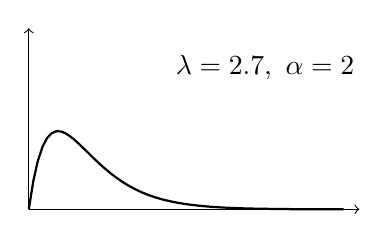
\begin{tikzpicture}[x=1cm,y=1cm]
\draw[->](0,0)--(4.2,0);\draw[->](0,0)--(0,2.3);
\draw[thick,domain=0:4,samples=70] plot (\x,{7.29*\x*exp(-2.7*\x)});
\node at (3,1.8) {$\lambda=2.7,\ \alpha=2$};
\end{tikzpicture}\end{center}
\textbf{Dimostrazione 1.}
\[\mathbb E(X)=\mathbb E\left(\sum_{i=1}^{\alpha}X_i\right)=\sum_{i=1}^{\alpha}\mathbb E(X_i)=\frac\alpha\lambda,\qquad
\operatorname{Var}(X)=\operatorname{Var}\left(\sum_{i=1}^{\alpha}X_i\right)=\sum_{i=1}^{\alpha}\operatorname{Var}(X_i)=\frac\alpha{\lambda^2}.\]
\textbf{Dimostrazione 2.}
\begin{align*}
\mathbb E(X)&=\int_{-\infty}^{+\infty}x\frac{\lambda^\alpha}{\Gamma(\alpha)}x^{\alpha-1}e^{-\lambda x}\,dx\\
&=\int_0^{+\infty}\frac{\lambda^\alpha}{\Gamma(\alpha)}x^{(\alpha-1)+1}e^{-\lambda x}\,dx\\
&=\frac{\lambda^\alpha}{\Gamma(\alpha)}\frac{\Gamma(\alpha+1)}{\lambda^{\alpha+1}}
\underbrace{\int_0^{+\infty}\frac{\lambda^{\alpha+1}}{\Gamma(\alpha+1)}x^{(\alpha+1)-1}e^{-\lambda x}\,dx}_{1}=\frac\alpha\lambda,\\
\operatorname{Var}(X)&=\mathbb E(X^2)-\mathbb E(X)^2
=\frac{\alpha^2+\alpha}{\lambda^2}-\frac{\alpha^2}{\lambda^2}=\frac\alpha{\lambda^2}.
\end{align*}
% Pagina originale 32
\pagina{32}
\begin{align*}
\mathbb E(X^2)&=\int_0^{+\infty}x^2\frac{\lambda^\alpha}{\Gamma(\alpha)}x^{\alpha-1}e^{-\lambda x}\,dx\\
&=\frac{\lambda^\alpha}{\Gamma(\alpha)}\frac{\Gamma(\alpha+2)}{\lambda^{\alpha+2}}
\int_0^{+\infty}\frac{\lambda^{\alpha+2}}{\Gamma(\alpha+2)}x^{(\alpha+2)-1}e^{-\lambda x}\,dx
=\frac{\alpha(\alpha+1)}{\lambda^2}.
\end{align*}
\textbf{Teorema.} $X\sim\operatorname{Gamma}(\alpha,\lambda)$, $Y\sim\operatorname{Gamma}(\beta,\lambda)$:
\[X+Y\sim\operatorname{Gamma}(\alpha+\beta,\lambda).\]
\subsection*{Legge normale}
$X\sim\mathcal N(\mu,\sigma^2)$, $\mu\in\mathbb R$, $\sigma^2\ge0$.
La somma di $n>30$ variabili $X_i$ i.i.d. porta ad una legge normale (teorema del limite centrale).
\[\boxed{f_X(x)=\frac1{\sigma\sqrt{2\pi}}e^{-\frac12((x-\mu)/\sigma)^2}}\quad X\sim\mathcal N(\mu,\sigma^2),\]
\[f_X(x)=\frac1{\sqrt{2\pi}}e^{-x^2/2}\quad X\sim\mathcal N(0,1).\]
\[\boxed{\mathbb E(X)=\mu,\quad\operatorname{Var}(X)=\sigma^2}\quad\text{per definizione}.\]
\begin{center}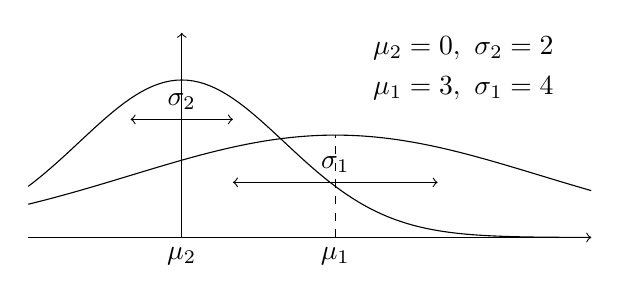
\begin{tikzpicture}[x=.65cm,y=1cm]
\draw[->](-3,0)--(8,0);\draw[->](0,0)--(0,2.6);
\draw[domain=-3:8,samples=100] plot(\x,{2*exp(-\x*\x/8)});
\draw[domain=-3:8,samples=100] plot(\x,{1.3*exp(-(\x-3)*(\x-3)/32)});
\draw[dashed](3,0)--(3,1.3);\node[below] at(0,0){$\mu_2$};\node[below] at(3,0){$\mu_1$};
\node at(5.5,2.4){$\mu_2=0,\ \sigma_2=2$};\node at(5.5,1.9){$\mu_1=3,\ \sigma_1=4$};
\draw[<->](-1,1.5)--(1,1.5) node[midway,above]{$\sigma_2$};\draw[<->](1,.7)--(5,.7)node[midway,above]{$\sigma_1$};
\end{tikzpicture}\end{center}
\[F_X(x)=\Phi(x)\quad\text{per }X\sim\mathcal N(0,1).\]
\textit{z-value}: $z=(x-\mu)/\sigma$ (quante deviazioni standard dista $x$ da $\mu$).
\textbf{Proprietà.} $X\sim\mathcal N(\mu,\sigma^2)$, $Y\sim\mathcal N(\nu,\tau^2)$:
\begin{gather*}
X+Y\sim\mathcal N(\mu+\nu,\sigma^2+\tau^2),\quad X+k\sim\mathcal N(\mu+k,\sigma^2),\\
aX\sim\mathcal N(a\mu,a^2\sigma^2),\quad aX+k\sim\mathcal N(a\mu+k,a^2\sigma^2).
\end{gather*}
% Pagina originale 33
\pagina{33}
\section*{Statistica inferenziale}
\textbf{Definizione.} Un vettore aleatorio $X'=(X_1,X_2,\ldots,X_n)$ composto da variabili aleatorie i.i.d. si chiama \emph{campione casuale}.

\textbf{Definizione.} I dati di un campione casuale $(X_1,X_2,\ldots,X_n)$ sono\[ (x_1,x_2,\ldots,x_n)\in R(X_1,X_2,\ldots,X_n).\]
$X$ è definita da parametri $\theta\in\Theta$.
\[X\sim\operatorname{Be}(p)\Rightarrow\theta=p,\quad\Theta=[0,1];\qquad
X\sim B(n,p)\Rightarrow\theta=(n,p),\quad\Theta=\mathbb N\times[0,1].\]
\subsection*{Obiettivo della statistica inferenziale}
Preso un campione casuale $(X_1,X_2,\ldots,X_n)$ della popolazione $X$, definita dai parametri $\theta\in\Theta$, l'obiettivo della statistica inferenziale è quello di ottenere informazioni sulla popolazione a partire dai dati $(x_1,\ldots,x_n)$ (questo processo è detto ``di inferenza'').

\textbf{Definizione.} Sia $(X_1,\ldots,X_n)$ un campione casuale. Una \emph{statistica} costruita a partire dal campione è una variabile aleatoria $H(X_1,\ldots,X_n)$.

\textbf{Esempio.} La media campionaria è la statistica $\overline X_n$:
\[\boxed{\overline X_n=\frac1n\sum_{i=1}^n X_i}.\]
$\overline x_n$ è la realizzazione di $\overline X_n$ calcolata sui dati:
\[\overline x_n=\frac1n\sum_{i=1}^n x_i.\]
Se la popolazione $X$ è definita da parametri $\theta\in\Theta$, $h(\theta)$ il parametro da stimare e $H(X_1,\ldots,X_n)$ ha lo scopo di stimare $h(\theta)$, allora $H(X_1,\ldots,X_n)$ è uno \emph{stimatore} di $h(\theta)$.
% Pagina originale 34
\pagina{34}
\textbf{Definizione.} Uno stimatore si dice \emph{corretto} se $H(X_1,\ldots,X_n)$ ha come valore atteso $h(\theta)$:
\[\mathbb E\bigl(H(X_1,\ldots,X_n)\bigr)=h(\theta).\]
$H(x_1,\ldots,x_n)$ si dice \emph{stima puntuale} di $h(\theta)$.

\textbf{Esempio.} La varianza campionaria è la statistica $S_n^2$:
\[\boxed{S_n^2=\frac1{n-1}\sum_i(X_i-\overline X_n)^2}.\]
\[s_n^2=\frac1{n-1}\sum_i(x_i-\overline x_n)^2\quad\text{è la realizzazione sui dati}.\]
\textbf{Osservazione.}
\[\boxed{\mathbb E(\overline X_n)=\mu,\qquad\operatorname{Var}(\overline X_n)=\frac{\sigma^2}{n}\ne\sigma^2}.\]
Con $n\to+\infty$, $\operatorname{Var}(\overline X_n)\to0$ (sempre più certa): legge dei grandi numeri.
\subsection*{Legge dei grandi numeri}
Siano $X_1,\ldots,X_n$ i.i.d. con $\mathbb E(X_i)=\mu$ e $\operatorname{Var}(X_i)=\sigma^2$:
\[\forall\varepsilon>0,\qquad\lim_{n\to+\infty}\mathbb P\{|\overline X_n-\mu|<\varepsilon\}=1.\]
\textbf{Dimostrazione.}
\[\mathbb P\{|\overline X_n-\mu|>\varepsilon\}=1-\mathbb P\{|\overline X_n-\mu|<\varepsilon\}\longrightarrow0.\]
Ponendo $Y=(\overline X_n-\mu)^2$:
\begin{align*}
\mathbb P\{|\overline X_n-\mu|>\varepsilon\}&=\mathbb P\{(\overline X_n-\mu)^2>\varepsilon^2\}
=\int_{\varepsilon^2}^{+\infty}f_Y(y)\,dy\\
&=\int_{\varepsilon^2}^{+\infty}\frac{\varepsilon^2}{\varepsilon^2}f_Y(y)\,dy
\le\frac1{\varepsilon^2}\int_{\varepsilon^2}^{+\infty}y f_Y(y)\,dy\\
&\le\frac1{\varepsilon^2}\int_0^{+\infty}y f_Y(y)\,dy
=\frac1{\varepsilon^2}\mathbb E(Y)=\frac1{\varepsilon^2}\mathbb E\bigl((\overline X_n-\mu)^2\bigr)\\
&=\frac1{\varepsilon^2}\left[\operatorname{Var}(\overline X_n-\mu)+\mathbb E(\overline X_n-\mu)^2\right]
=\frac1{\varepsilon^2}\left(\frac{\sigma^2}{n}+0^2\right)=\frac{\sigma^2}{\varepsilon^2 n}\longrightarrow0.
\end{align*}
% Pagina originale 35
\pagina{35}
Dalla legge dei grandi numeri nasce la \emph{simulazione di Montecarlo}.
Sapendo che con $n\to+\infty$ tentativi $\overline X_n\to\mu$, possiamo usare un calcolatore per simulare $n$ tentativi e trovare $\mu$.
\textbf{Esempio.} Simulazione Montecarlo per $\pi$.
\begin{center}\begin{tikzpicture}\draw (0,0) rectangle(2,2);\draw[fill=gray!20](1,1)circle(1);\node[right]at(2.4,1){$\pi=4\,\dfrac{\#\text{successi}}{\#\text{tentativi}}$};\end{tikzpicture}\end{center}
\[\#\text{successi}=A_{\circ}=\pi(1/2)^2=\pi/4,\quad\#\text{tentativi}=A_{\square}=1^2=1,\quad\mu\to\pi/4.\]
\subsection*{Teorema del limite centrale}
Sia $X$ popolazione con $\mathbb E(X)=\mu$ e $\operatorname{Var}(X)=\sigma^2$, $X_1,\ldots,X_n$ i.i.d.:
\[\lim_{n\to+\infty}\mathbb P\left\{\frac{\overline X_n-\mu}{\sigma/\sqrt n}\le z\right\}=\Phi(z)=\frac1{\sqrt{2\pi}}\int_{-\infty}^z e^{-t^2/2}\,dt.\]
Applicabile per $n\ge30$ senza aver bisogno di conoscere la legge di $X_i$.
\subsection*{Intervalli di confidenza (I.C.)}
Un I.C. con livello di confidenza $\beta$ è un intervallo aleatorio $[U_n,V_n]$, dove $U_n=u_n(X_1,\ldots,X_n)$ e $V_n=v_n(X_1,\ldots,X_n)$ sono statistiche, tali che
\[\boxed{\beta=\mathbb P\{U_n\le h(\theta)\le V_n\}}.\]
\textbf{Esempio.} $h(\theta)=\mu$ ($\sigma$ noto):
\begin{align*}
\beta&=\mathbb P\{U_n\le\mu\le V_n\}=\mathbb P\{-V_n\le-\mu\le-U_n\}\\
&=\mathbb P\left\{\frac{\overline X_n-V_n}{\sigma/\sqrt n}\le
\underbrace{\frac{\overline X_n-\mu}{\sigma/\sqrt n}}_{Z\sim\mathcal N(0,1)}\le\frac{\overline X_n-U_n}{\sigma/\sqrt n}\right\}.
\end{align*}
% Pagina originale 36
\pagina{36}
\begin{align*}
\beta&=1-\mathbb P\left(\left\{Z\le\frac{\overline X_n-V_n}{\sigma/\sqrt n}\right\}\cup
\left\{Z\ge\frac{\overline X_n-U_n}{\sigma/\sqrt n}\right\}\right)\\
&=1-2\underbrace{\mathbb P\{Z\ge z_{\alpha/2}\}}_{\alpha/2},\qquad\alpha=1-\beta.
\end{align*}
\[(1-2\alpha/2=1-\alpha=\beta).\]
\begin{gather*}
\frac{\overline X_n-V_n}{\sigma/\sqrt n}=-z_{\alpha/2}\Rightarrow V_n=\overline X_n+\frac\sigma{\sqrt n}z_{\alpha/2},\\
\frac{\overline X_n-U_n}{\sigma/\sqrt n}=z_{\alpha/2}\Rightarrow U_n=\overline X_n-\frac\sigma{\sqrt n}z_{\alpha/2},\\
\boxed{\mathrm{I.C.}=\left[\overline X_n-z_{\alpha/2}\frac\sigma{\sqrt n},\ \overline X_n+z_{\alpha/2}\frac\sigma{\sqrt n}\right]},\\
z_{\alpha/2}=\Phi^{-1}(1-\alpha/2),\qquad[z_x=\Phi^{-1}(1-x)],\qquad[\Phi(x)+\Phi(-x)=1].
\end{gather*}
\begin{center}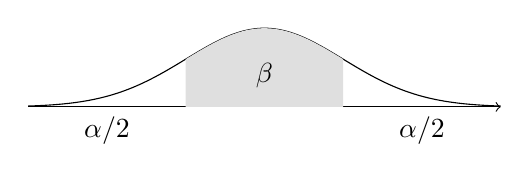
\begin{tikzpicture}[x=1cm,y=1cm]\draw[->](-3,0)--(3,0);\draw[domain=-3:3,samples=80]plot(\x,{exp(-\x*\x/2)});\fill[gray!25,domain=-1:1,samples=40](-1,0)--plot(\x,{exp(-\x*\x/2)})--(1,0)--cycle;\node at(0,.4){$\beta$};\node[below]at(-2,0){$\alpha/2$};\node[below]at(2,0){$\alpha/2$};\end{tikzpicture}\end{center}
\textbf{Esempio.} $h(\theta)=\sigma^2$:
\begin{align*}
\beta&=\mathbb P\{U_n\le\sigma^2\le V_n\}=\mathbb P\{1/V_n\le1/\sigma^2\le1/U_n\}\\
&=\mathbb P\left\{\frac{(n-1)S_n^2}{V_n}\le\underbrace{\frac{(n-1)S_n^2}{\sigma^2}}_{Z\sim\chi^2(n-1)}\le\frac{(n-1)S_n^2}{U_n}\right\}.
\end{align*}
\begin{gather*}
\frac{(n-1)S_n^2}{V_n}=\chi^2_{n-1,1-\alpha/2}\Rightarrow V_n=\frac{(n-1)S_n^2}{\chi^2_{n-1,1-\alpha/2}},\\
\frac{(n-1)S_n^2}{U_n}=\chi^2_{n-1,\alpha/2}\Rightarrow U_n=\frac{(n-1)S_n^2}{\chi^2_{n-1,\alpha/2}},\\
\boxed{\mathrm{I.C.}=\left[\frac{(n-1)S_n^2}{\chi^2_{n-1,\alpha/2}},\ \frac{(n-1)S_n^2}{\chi^2_{n-1,1-\alpha/2}}\right]}.
\end{gather*}
\emph{Nota di trascrizione: nell'originale, due indici nella derivazione di $V_n$ sembrano scritti $1+\alpha/2$; il riquadro finale riporta $1-\alpha/2$. Qui è seguito il riquadro. I quantili sono indicati secondo la convenzione di coda destra.}
\begin{center}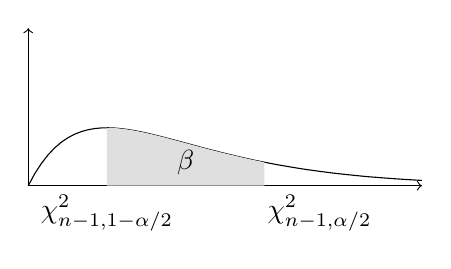
\begin{tikzpicture}\draw[->](0,0)--(5,0);\draw[->](0,0)--(0,2);\draw[domain=0:5,samples=60]plot(\x,{2*\x*exp(-\x)});\fill[gray!25,domain=1:3,samples=30](1,0)--plot(\x,{2*\x*exp(-\x)})--(3,0)--cycle;\node at(2,.3){$\beta$};\node[below]at(1,0){$\chi^2_{n-1,1-\alpha/2}$};\node[below]at(3.7,0){$\chi^2_{n-1,\alpha/2}$};\end{tikzpicture}\end{center}
% Pagina originale 37
\pagina{37}
\textbf{Esempio.} $h(\theta)=\mu$ ($\sigma$ non noto):
\[\beta=\mathbb P\{U_n\le\mu\le V_n\}
=\mathbb P\left\{\frac{\overline X_n-V_n}{S_n/\sqrt n}\le\underbrace{\frac{\overline X_n-\mu}{S_n/\sqrt n}}_{\sim t(n-1)}\le\frac{\overline X_n-U_n}{S_n/\sqrt n}\right\}.\]
\section*{Leggi continue per analisi inferenziale}
\subsection*{Chi-quadro}
$X\sim\chi^2(n)$:
\[\chi^2(n)=\operatorname{Gamma}(n/2,1/2),\qquad
\boxed{f_X(x)=\frac{\lambda^{n/2}}{\Gamma(n/2)}x^{n/2-1}e^{-x/2}}\quad(\lambda=1/2).\]
\begin{center}\begin{tikzpicture}\draw[->](0,0)--(5,0);\draw[->](0,0)--(0,2);\draw[domain=0.01:5,samples=80]plot(\x,{1.5*sqrt(\x)*exp(-\x/2)});\node at(4,1.5){$n=3$};\end{tikzpicture}\end{center}
\textbf{Osservazione.} $\sum_{i=1}^n X_i^2=Z\sim\operatorname{Gamma}(n/2,1/2)$, $X_i\sim\mathcal N(0,1)$.
\textbf{Dimostrazione.} $f_{Z^2}(x)=?$ (qui $Z$ indica una normale standard).
\begin{align*}
\mathbb P\{Z^2\le x\}&=0\quad\forall x\le0,\\
\mathbb P\{Z^2\le x\}&=\mathbb P\{-\sqrt x\le Z\le\sqrt x\}=2\mathbb P\{0\le Z\le\sqrt x\}\\
&=2\int_0^{\sqrt x}\frac1{\sqrt{2\pi}}e^{-t^2/2}\,dt
\quad(y=t^2)\\
&=2\int_0^x\frac1{\sqrt{2\pi}}\frac1{2\sqrt y}e^{-y/2}\,dy=F_{Z^2}(x),\\
F'_{Z^2}(x)&=f_{Z^2}(x)=\frac1{\sqrt{2\pi}}\frac1{\sqrt x}e^{-x/2}
=\frac{(1/2)^{1/2}}{\underbrace{\Gamma(1/2)}_{\sqrt\pi}}x^{1/2-1}e^{-x/2}.
\end{align*}
\textbf{Perché si usa?}
\begin{align*}
S_n^2&=\frac1{n-1}\sum_{i=1}^n(X_i-\overline X_n)^2\\
&=\frac1{n-1}\sum_{i=1}^n\left[(X_i-\mu)^2+(\overline X_n-\mu)^2-2(X_i-\mu)(\overline X_n-\mu)\right]\\
&=\frac1{n-1}\left[\sum_{i=1}^n(X_i-\mu)^2+n(\overline X_n-\mu)^2-2(\overline X_n-\mu)(n\overline X_n-n\mu)\right].
\end{align*}
% Pagina originale 38
\pagina{38}
\begin{align*}
S_n^2&=\frac1{n-1}\left[\sum_{i=1}^n(X_i-\mu)^2-n(\overline X_n-\mu)^2\right],\\
(n-1)S_n^2&=\sum_{i=1}^n(X_i-\mu)^2-n(\overline X_n-\mu)^2,\\
\frac{(n-1)S_n^2}{\sigma^2}+n\left(\frac{\overline X_n-\mu}{\sigma}\right)^2&=\sum_{i=1}^n\left(\frac{X_i-\mu}{\sigma}\right)^2,\\
\frac{(n-1)S_n^2}{\sigma^2}+\underbrace{\left(\frac{\overline X_n-\mu}{\sigma/\sqrt n}\right)^2}_{Z_0^2,\ Z_0\sim\mathcal N(0,1)}&=\sum_{i=1}^n\underbrace{\left(\frac{X_i-\mu}{\sigma}\right)^2}_{Z_i^2,\ Z_i\sim\mathcal N(0,1)},\\
\frac{(n-1)S_n^2}{\sigma^2}+Z_0^2&=\sum_{i=1}^n Z_i^2.
\end{align*}
\begin{gather*}
Z_0^2\sim\chi^2(1)=\operatorname{Gamma}(1/2,1/2),\quad Z_i^2\sim\chi^2(1)=\operatorname{Gamma}(1/2,1/2),\\
\sum Z_i^2\sim\chi^2(n)=\operatorname{Gamma}(n/2,1/2),\\
\Rightarrow\frac{(n-1)S_n^2}{\sigma^2}\sim\operatorname{Gamma}((n-1)/2,1/2)=\chi^2(n-1).
\end{gather*}
\subsection*{t-Student}
$X\sim t(n)$:
\[X=\frac Z{\sqrt{Q_n/n}},\qquad Z\sim\mathcal N(0,1),\quad Q_n\sim\chi^2(n).\]
\[\boxed{f_X(x)=\frac{\Gamma((n+1)/2)}{\sqrt{n\pi}\,\Gamma(n/2)}\frac1{(1+x^2/n)^{(n+1)/2}}}.\]
\[n\to+\infty\Rightarrow X\sim t(n)\approx\mathcal N(0,1).\]
\textbf{Perché si usa?}
\begin{align*}
\frac{\overline X_n-\mu}{S_n/\sqrt n}&=\frac{\overline X_n-\mu}{\sigma/\sqrt n}\frac\sigma{S_n}
=\underbrace{Z}_{\sim\mathcal N(0,1)}\frac1{\sqrt{S_n^2/\sigma^2}}\frac{\sqrt{n-1}}{\sqrt{n-1}}\\
&=Z\frac{\sqrt{n-1}}{\sqrt{(n-1)S_n^2/\sigma^2}}
=\frac Z{\sqrt{Q_{n-1}/(n-1)}}\sim t(n-1),\quad Q_{n-1}=\frac{(n-1)S_n^2}{\sigma^2}\sim\chi^2(n-1).
\end{align*}
% Pagina originale 39
\pagina{39}
\subsection*{Intervallo di confidenza unilaterale}
\[\boxed{\beta=\mathbb P\{U_n\le h(\theta)\}}\quad\text{limite inferiore di confidenza }U_n,\]
\[\boxed{\beta=\mathbb P\{h(\theta)\le V_n\}}\quad\text{limite superiore di confidenza }V_n.\]
\textbf{Nota.} In questo caso viene preso $z_\alpha$ e non $z_{\alpha/2}$.
\subsection*{Test di ipotesi}
Si parte da un'ipotesi nulla $H_0:h(\theta)\in E_0$ e si verifica che l'ipotesi alternativa $H_1:h(\theta)\in E_1$, con $E_0\cap E_1=\varnothing$, è rifiutabile o accettabile secondo il livello di significatività $\alpha\in(0,1)$.
\textbf{Errori.}
\begin{center}\begin{tabular}{c|cc}&$H_0$ vera&$\overline H_0$ vera\\\hline
Accettare $H_0$&corretto&II tipo\\Rifiutare $H_0$&I tipo&corretto\end{tabular}\end{center}
I tipo: $\mu=3$ ($H_0$), ma pensiamo che $\mu>3$ ($H_1$).
II tipo: $\mu>3$ ($H_1$), ma pensiamo che $\mu=3$ ($H_0$).
Il livello di significatività $\alpha$ è la probabilità di commettere un errore del I tipo.
\[\boxed{R_c=\{(x_1,\ldots,x_n)\in R(X_1,\ldots,X_n):\overline x_n>\mu_0+\delta\}},\]
\[\boxed{\alpha=\mathbb P\{(X_1,\ldots,X_n)\in R_c\}}\quad\text{essendo vera }\mu=\mu_0.\]
\begin{align*}
\alpha&=\mathbb P\{\overline X_n>\mu_0+\delta\}
=\mathbb P\left\{\frac{\overline X_n-\mu}{\sigma/\sqrt n}>\frac{\mu_0-\mu}{\sigma/\sqrt n}+\frac\delta{\sigma/\sqrt n}\right\}\\
&=\mathbb P\left\{\underbrace{Z}_{\sim\mathcal N(0,1)}>\frac\delta{\sigma/\sqrt n}\right\}\quad(\mu=\mu_0).
\end{align*}
\[\frac\delta{\sigma/\sqrt n}=z_\alpha\Rightarrow\delta=\frac\sigma{\sqrt n}z_\alpha.\]
Se $\overline x_n>\mu_0+\delta=\mu_0+\frac\sigma{\sqrt n}z_\alpha$, allora $H_0$ è rifiutata.
% Pagina originale 40
\pagina{40}
\textbf{Osservazione.} Se $H_0$ è rifiutata con livello di significatività $\alpha'$, allora $H_0$ è rifiutata con $\alpha>\alpha'$.
\subsection*{p-value}
Il p-value è il più piccolo livello di significatività $\alpha$ per cui i dati permettono di rifiutare l'ipotesi nulla $H_0$.
\[\forall\alpha>\text{p-value}:H_0\text{ è rifiutata};\qquad\forall\alpha<\text{p-value}:H_0\text{ è accettata}.\]
\begin{align*}
\text{p-value}&=\inf\left\{\alpha\in(0,1):\overline x_n>\mu_0+\frac\sigma{\sqrt n}z_\alpha\right\}\\
&=\inf\left\{\alpha\in(0,1):\underbrace{\frac{\overline x_n-\mu_0}{\sigma/\sqrt n}}_{\text{z-score}}>z_\alpha\right\}\\
&=\inf_{\alpha\in(0,1)}\left\{\Phi(z_\alpha)<\Phi\left(\frac{\overline x_n-\mu_0}{\sigma/\sqrt n}\right)\right\}\\
&=\inf_{\alpha\in(0,1)}\left\{1-\alpha<\Phi\left(\frac{\overline x_n-\mu_0}{\sigma/\sqrt n}\right)\right\}\\
&=\inf_{\alpha\in(0,1)}\left\{\alpha>1-\Phi\left(\frac{\overline x_n-\mu_0}{\sigma/\sqrt n}\right)\right\}
=1-\Phi\left(\frac{\overline x_n-\mu_0}{\sigma/\sqrt n}\right)=\Phi(-\text{z-value}).
\end{align*}
